\section{Decision tree}

% ----- Q.1 ----- %
\subsection{Effect of the tree depth on the decision boundary}

% ----- Q.1.a
\subsubsection{{\it Illustrate and explain the decision boundary for each depth}}
We built several decision tree models with different depth values, for both datasets. To illustrate our results, we present the decision boundary of each model at figures \ref{fig:dt_make_data1} (for dataset 1) and \ref{fig:dt_make_data2} (for dataset 2).\par
In order to make the visualization clearer, we only displayed \num{25}\% of the points of each testing set and did not include the depth of 8, as the decision boundary is almost identical to the unconstrained depth one.\par
On every plot (not just for this section, but for the whole report), an accuracy is associated with each decision boundary. It is computed on the whole testing set (\num{1850} points).\par
Firstly, we can see that, in all cases, the model partitions the features space along the axes. This result is logical considering the operation of the algorithm : it splits the dataset by thresholding the value of one of the features.\par
Secondly, we find that, as the depth of the tree increases, the number of partitions of the space increases exponentially. This result is also logical: incrementing the depth of a tree by 1 increases exponentially the total number of nodes since each node at depth $d-1$ is sub-divided into usually two (in this algorithm) nodes.
\begin{figure}[H]
    \centering
    \begin{subfigure}{0.495\textwidth}
        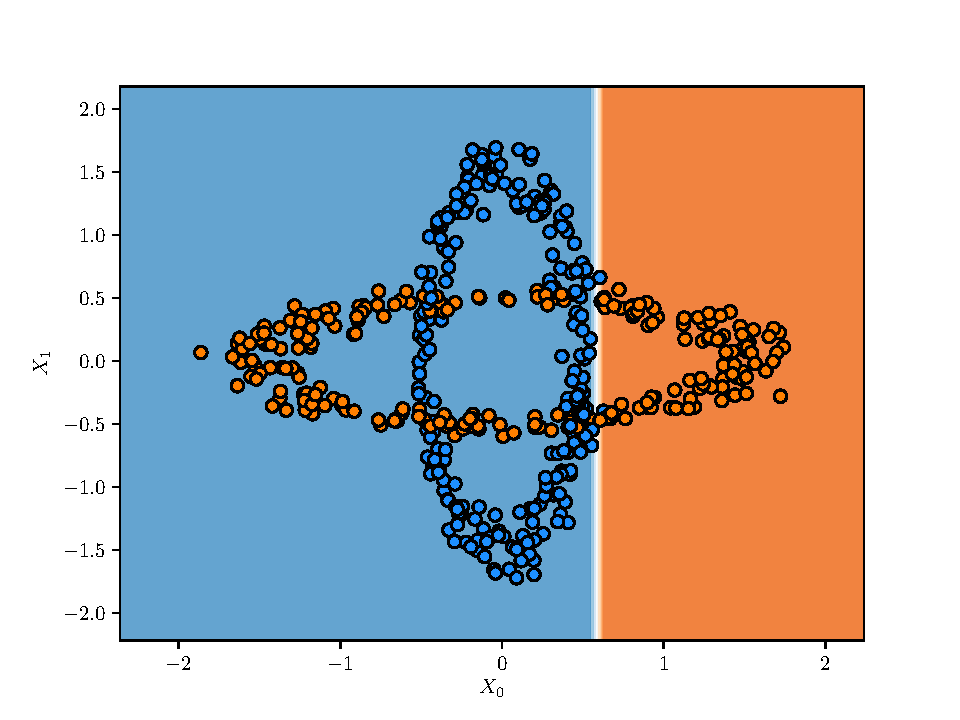
\includegraphics[width=\textwidth]{resources/pdf/make_data1_dt_1.pdf}
        \caption{Decision tree : depth of 1 (acc = \num{0.68})}
    \end{subfigure}
    \begin{subfigure}{0.495\textwidth}
        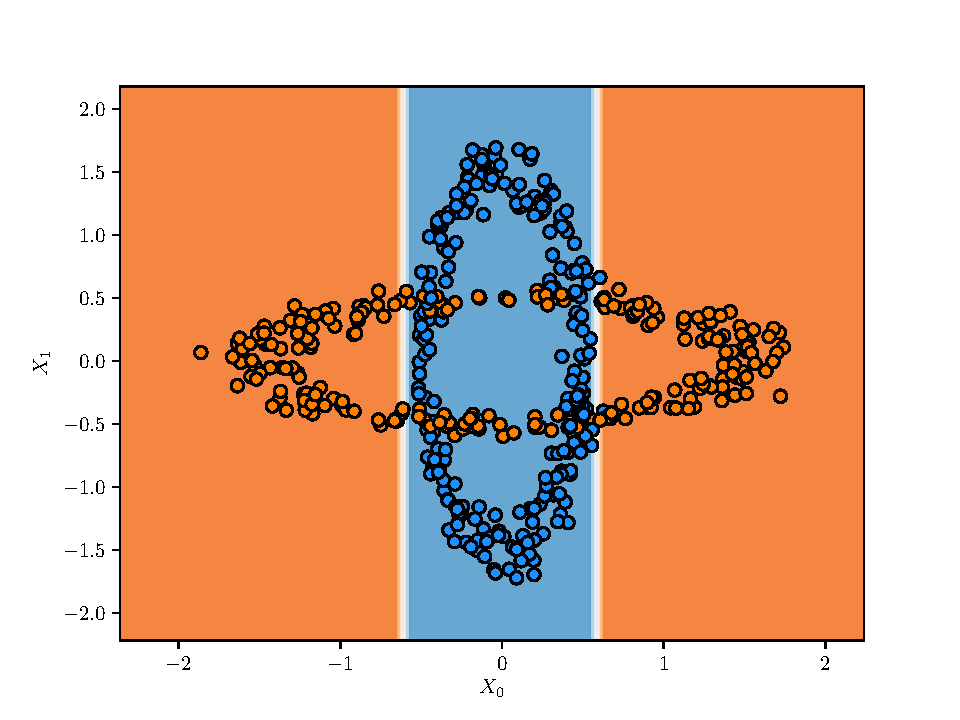
\includegraphics[width=\textwidth]{resources/pdf/make_data1_dt_2.pdf}
        \caption{Decision tree : depth of 2 (acc = \num{0.87})}
    \end{subfigure}
    \vspace{3pt}
    \begin{subfigure}{0.495\textwidth}
        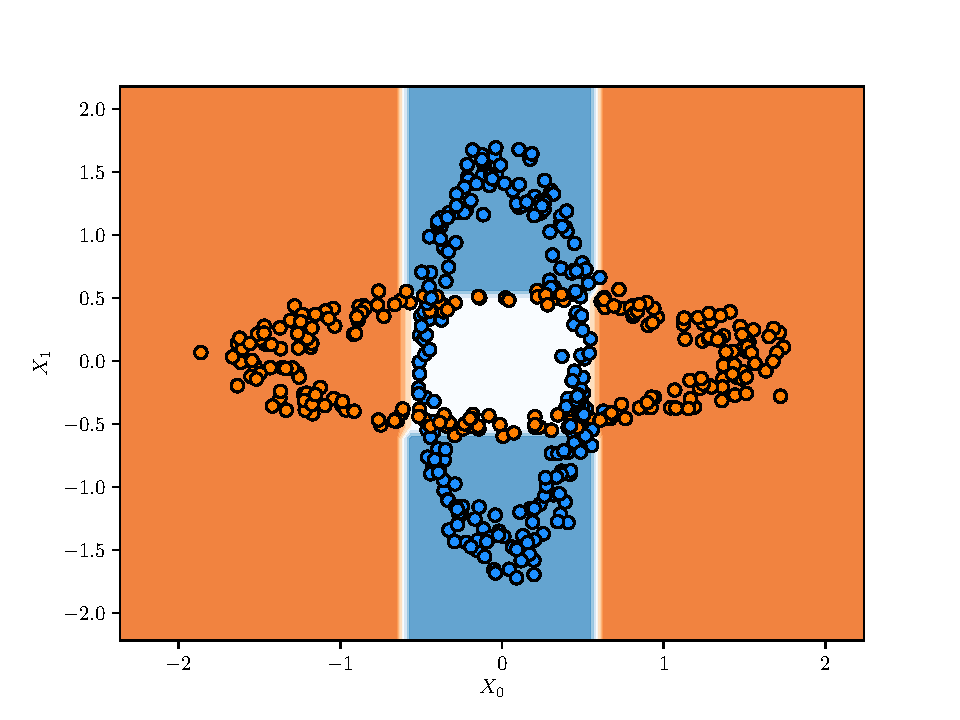
\includegraphics[width=\textwidth]{resources/pdf/make_data1_dt_4.pdf}
        \caption{Decision tree : depth of 4 (acc = \num{0.86})}
    \end{subfigure}
    \begin{subfigure}{0.495\textwidth}
        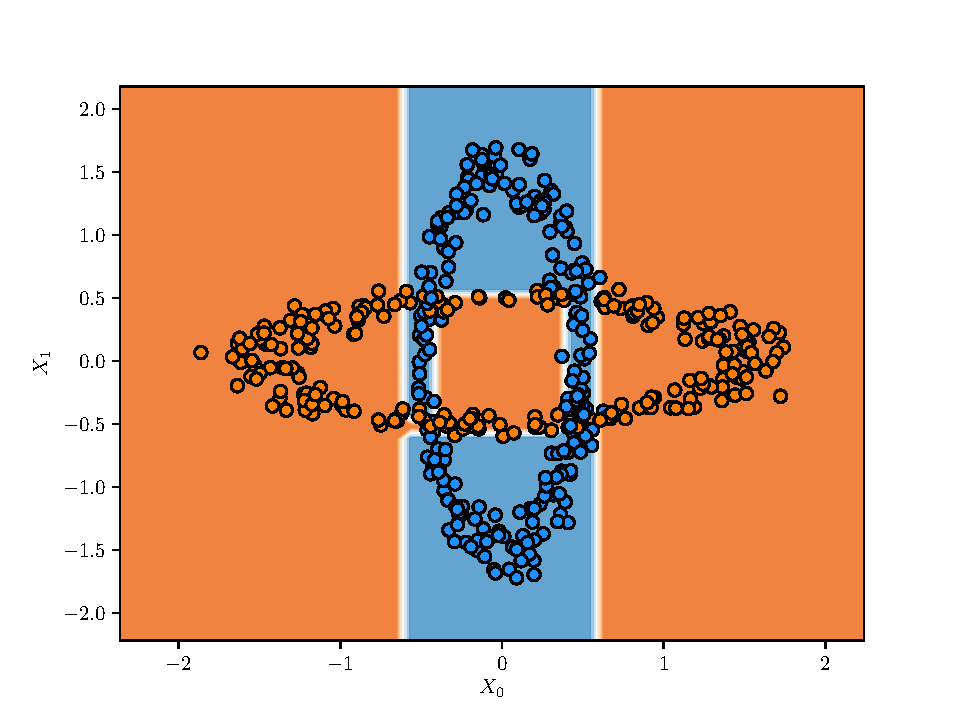
\includegraphics[width=\textwidth]{resources/pdf/make_data1_dt_None.pdf}
        \caption{Decision tree : unconstrained (acc = \num{0.93})}
    \end{subfigure}
    \noskipcaption{Decision tree boundary for several depths using \texttt{make\_data1}}
    \label{fig:dt_make_data1}
\end{figure}
\begin{comment}

Regarding the results of dataset 1 presented in figure \ref{fig:dt_make_data1}, we observe that, for depths of 1 and 2, we have underfitting : the delimited zones are too simple to classify the data in an acceptable way. For a depth of 1, the decision boundary is only affected by the value of one feature and is therefore too simplistic.\par
For greater depths (4 and more), the results seem to improve : the areas are refined and become more precise. However, for depths of 8 and above (including unconstrained depth), overfitting is observed : the model has too many small specific regions at a few specific points.\par
\end{comment}

Regarding the results of dataset 1 presented in figure \ref{fig:dt_make_data1}, we observe that, for a depth of 1, we have a very poor classification of the data (only one splitting is performed). For a depth of 2, we have a better decision boundary that is composed of 3 zones (the maximum for that depth would be 4). As the depth increases, the results improve. The areas are refined and become more precise but, as will be explained later, we begin to see overfitting. It is worth noting that the maximal possible number of zones for the decision boundary is $2^{\text{depth}}$, which is not observed for any depth above 1 for this dataset.

\begin{figure}[H]
    \centering
    \begin{subfigure}{0.495\textwidth}
        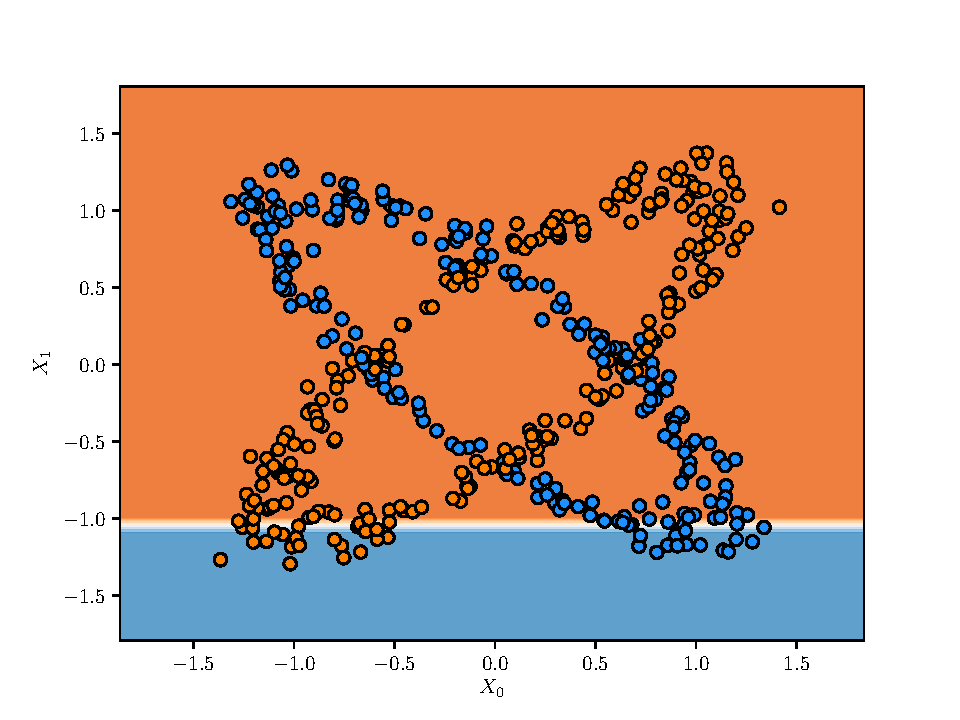
\includegraphics[width=\textwidth]{resources/pdf/make_data2_dt_1.pdf}
        \caption{Decision tree : depth of 1 (acc = \num{0.49})}
    \end{subfigure}
    \begin{subfigure}{0.495\textwidth}
        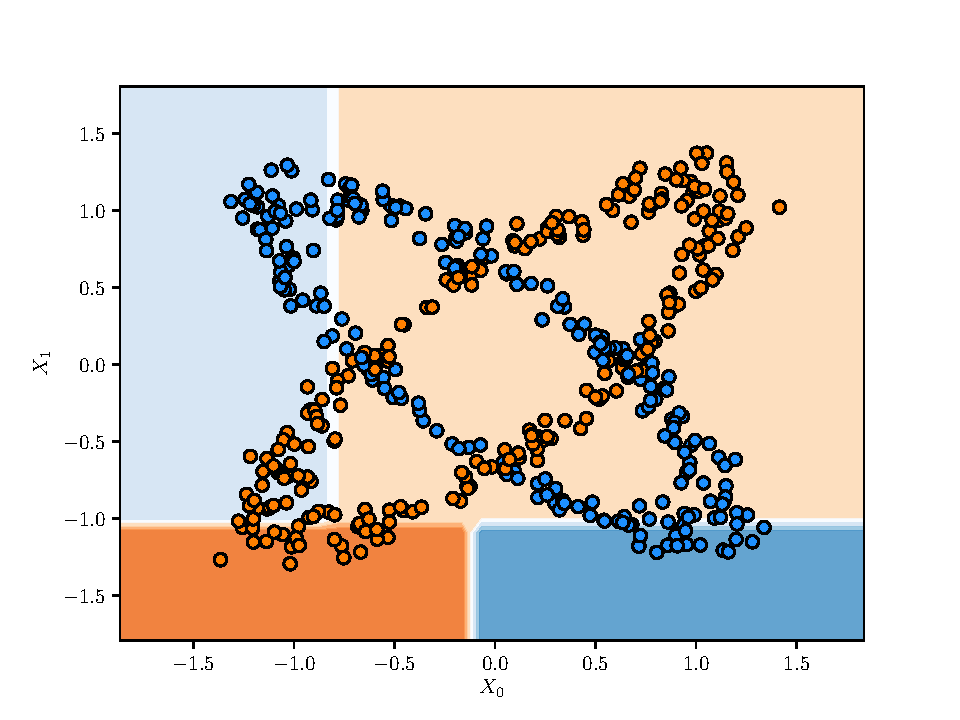
\includegraphics[width=\textwidth]{resources/pdf/make_data2_dt_2.pdf}
        \caption{Decision tree : depth of 2 (acc = \num{0.55})}
    \end{subfigure}
    \vspace{3pt}
    \begin{subfigure}{0.495\textwidth}
        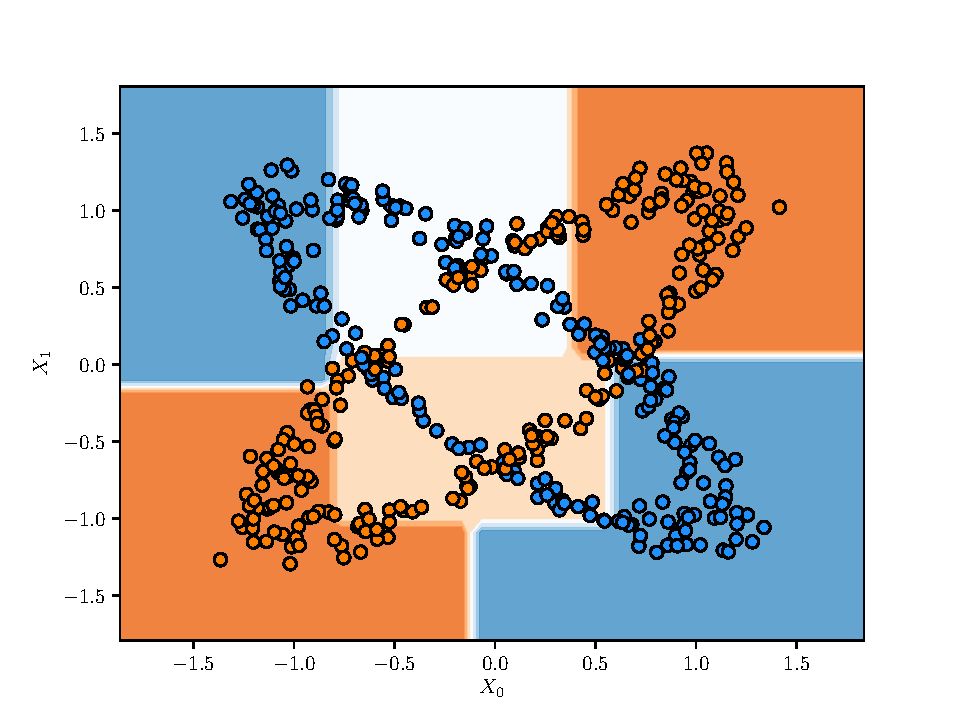
\includegraphics[width=\textwidth]{resources/pdf/make_data2_dt_4.pdf}
        \caption{Decision tree : depth of 4 (acc = \num{0.79})}
    \end{subfigure}
    \begin{subfigure}{0.495\textwidth}
        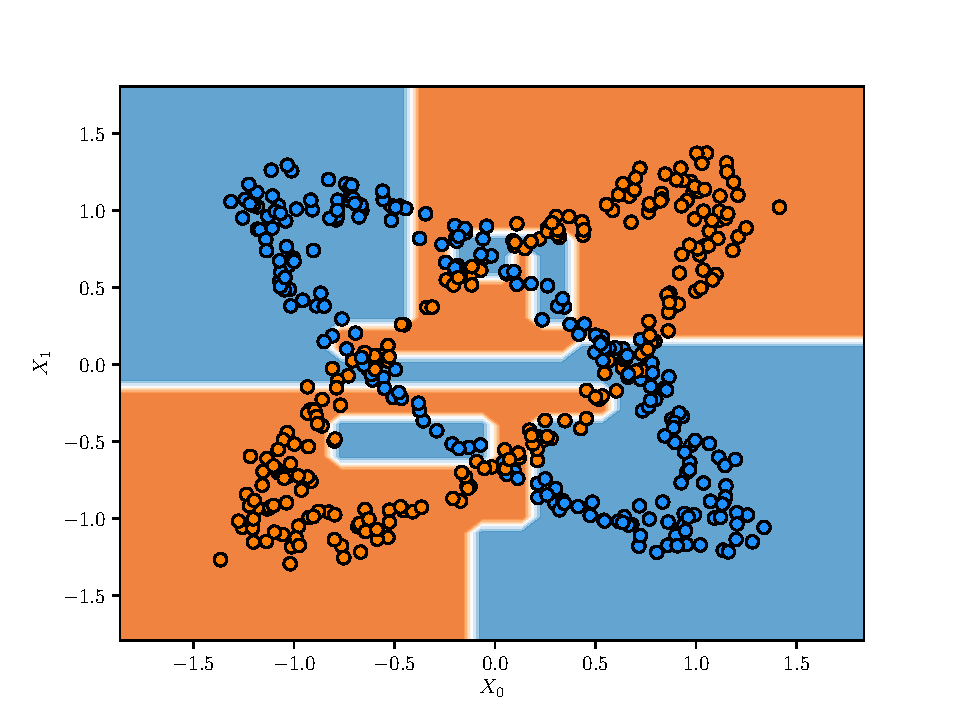
\includegraphics[width=\textwidth]{resources/pdf/make_data2_dt_None.pdf}
        \caption{Decision tree : unconstrained (acc = \num{0.83})}
    \end{subfigure}
    \noskipcaption{Decision tree boundary for several depths using \texttt{make\_data2}}
    \label{fig:dt_make_data2}
\end{figure}
\begin{comment}
Concerning dataset 2, the results are very similar to those of dataset 1. For shallow depths (1 and 2), the decisions are not very good : the borders are too simple to classify the data correctly, and for higher depths (more than 4), one begins to observe the overfitting.\par
The borders of the areas are more complex for dataset 2 than dataset 1. This is certainly due to the fact that the ellipses of dataset 1 are parallel to the axes and those of dataset 2 are not. Given the operation of the algorithm described previously, it certainly influences boundaries.\par
For both datasets, a tree of depth 4 seems to be the best classification model. It is certainly the model that lies between the limits of underfitting and overfitting.
\end{comment}

Concerning dataset 2, the results are very similar to those of dataset 1. For shallow depths (1 and 2), the decisions are not very good : the borders are too simple to classify the data correctly, and for higher depths (more than 4), one begins to observe the overfitting.\par
One difference with the first dataset is that the decision boundary is more complex in this case. This is certainly due to the fact that the ellipses of dataset 1 are parallel to the axes and those of dataset 2 are not, they cross the main axes at roughly $45°$ angle. Given the operation of the algorithm described previously (the splitting of the features space is performed parallel to the axes), the boundary must be more complex and is less satisfactory than for the first dataset.\par
For both datasets, a tree of depth 4 seems to be the best classification model. It is certainly the model that lies between the limits of underfitting and overfitting.

\begin{comment}
On the basis of the graphs given at figures \ref{fig:dt_make_data1} and \ref{fig:dt_make_data2}, for the \textbf{dataset 1}, 
\begin{itemize}
    \item For a \textbf{depth of 1}, we can see that the decision boundary is quite simple. Indeed, the decision is only affected by the value of one variable. \textbf{Compute accuracy to show that it is probably the best way to make a decision with a single decision node.}
    \item For a \textbf{depth of 2}, the decision process becomes a bit more advanced. For the first dataset, the cutting zone that was seen for the depth of 1 becomes symmetric along the $X_1$ axis. Indeed, with a depth of 2, we can refine the previous decision. If $X_1 > - 0.5$, discriminate the cases in which it is over $0.5$ or not. We therefore have 3 leaves. For the second dataset, we clearly see that a second split is performed for each elements after the first split. We therefore have 4 leaves. \textbf{As will be seen ..., it may be the best decision. Is it possible to easily prove that ? Ou alors c'est décidé par DTClassifier qui prend le premier argument comme cutting decision.}
    \item For a \textbf{depth of 4}, two new "questions" can be asked each time we have to make a categorization. When we take a look at the first dataset, it seems logical to discriminate the values of $X_0$ in the same kind of way as we did for $X_1$. The boundary is similar to what we have for a depth of 2, except, now, there is also a vertical delimitation. For the second dataset, the extension of the decision tree is more difficult to analyze, but the different categorization zones also become more numerous.
    \item For a \textbf{depth of 8}, the decision process is refined, and more tests, based on the values of the two parameters, can be made. We will not analyze it thoroughly as up to 7 (?) "questions can be asked for each sample to classify it".
    \item For an \textbf{unbounded depth}, we can see that it does not differ from the previous depth of 8, so it seems that the previous depth is the optimal depth given our (meager) training dataset.
\end{itemize}
\end{comment}

% ----- Q.1.b
\subsubsection{{\it Underfitting and overfitting}}
For both datasets, underfitting is clearly observed for a depth of 1 : a single two-zone delimitation is not sufficient to classify an acceptable number of data correctly. The very low accuracy compared to other depths is also evidence for the underfitting. For a depth of 2, the models improve. They still are not accurate enough, but we begin to have a good accuracy for the first dataset, although too many orange points lie in the blue zone (the decision for dataset 1 is only based on the value of one feature for this depth, which is not a good thing as the other feature is also correlated to the output). The boundary is still too simplistic for that depth to be used in practice.\par
For dataset 1, greater depths show better accuracies but, for depths of 8 and above, we clearly see some overfitting : the model has many small specific regions to try to have as good an accuracy on the training set as possible.\par
For the second dataset, we also begin to see overfitting for depths above 4, with many small regions appearing and feeling \og{}forced\fg{}, non natural, as for the first dataset. As said before, a depth of $4$ seems to lie between over- and underfitting.\par 

\paragraph{NB :} We plotted the errors for the training and testing sets as the depth increases, as shown during the lectures, to see where we have under- and overfitting. However, the testing set errors did not grew after a given point, they rather plateaued after a depth of 5 for the first dataset and a depth of 7 for the second, so we did not include these plots in our analysis.
\begin{comment}
\begin{itemize}
    \item \textbf{For dataset 1}, we can clearly see some underfitting for the depths of 1. The decision boundary is too simple and classifies a lot of orange points as blue.
\end{itemize}
Overfitting for 8 and none of dataset2, not for dataset1. Underfitting for lower depth, good for depth 4 of both datasets. \textbf{Quelles preuves ? Les petites zones qui s'étendent de manière non naturelle pour aller chercher des zones ?}
\end{comment}

% ----- Q.1.c
\subsubsection{{\it Why the model seems more confident when the depth is unconstrained ?}}
Because it perfectly classifies the training set (indeed, it can grow to the point where it only has one element per leaf). As the decision tree predicts for each zone the proportion of training objects that belong to that zone and as the zones are perfectly pure (only one class in them), the model is perfectly confident, although it usually overfits a lot.

% ----- Q.2 ----- %
\subsection{Average and standard deviation of test set accuracies}
The accuracies of the model for different depths were computed over 5 generations. The averages and variances of these accuracies are presented in figure \ref{fig:dt_accuracy}.
\begin{figure}[H]
    \centering
    \begin{subfigure}{0.495\textwidth}
        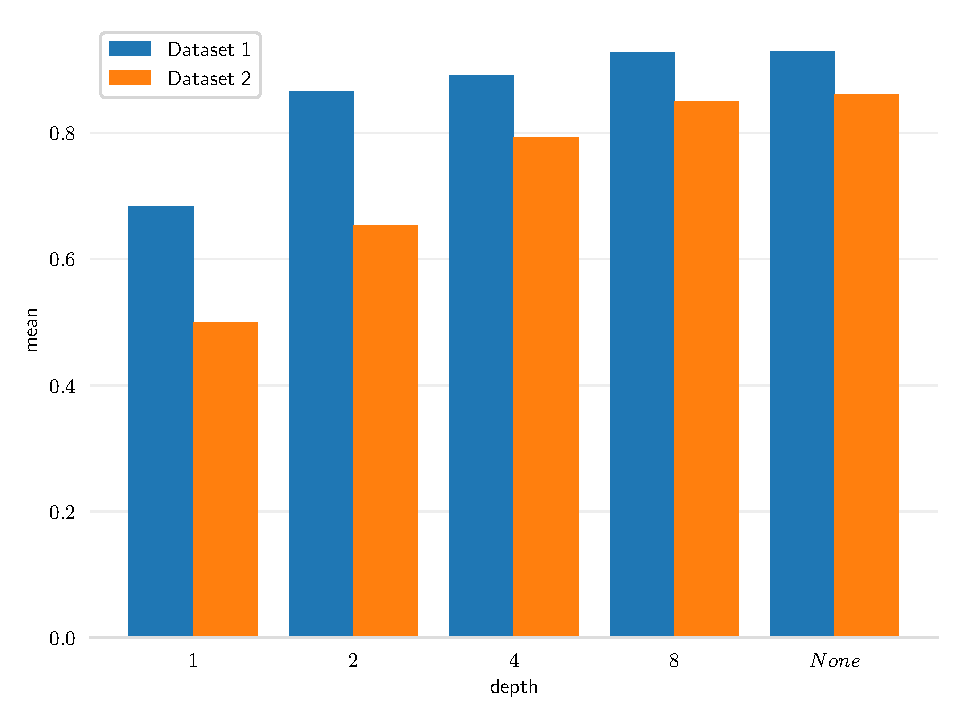
\includegraphics[width=\textwidth]{resources/pdf/dt_accuracies_mean.pdf}
        \caption{Average}
    \end{subfigure}
    \begin{subfigure}{0.495\textwidth}
        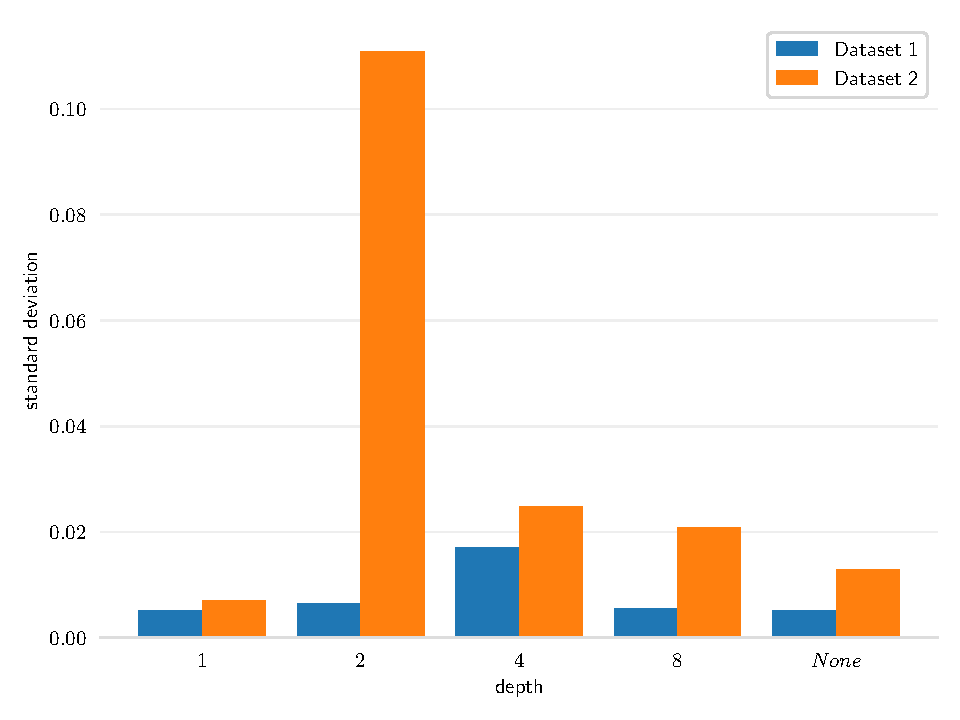
\includegraphics[width=\textwidth]{resources/pdf/dt_accuracies_std.pdf}
        \caption{Standard deviation}
    \end{subfigure}
    \noskipcaption{Statistics about test set accuracies over 5 generations}
    \label{fig:dt_accuracy}
\end{figure}
For the mean, the conclusion is the same for both dataset, although the overall accuracy is better for dataset 1, with the difference between the two datasets being greater for smaller depth (explained by the fact that a simple \og{}axis-following\fg{} classification yields better results for dataset 1 than dataset 2 as a consequence of the positions of the ellipses). The mean accuracy increases greatly as the depth increases, reaching high accuracy levels for the training set, but leading to overfitting, as was discussed above. We also see no increase in accuracy going from a depth of 8 to unconstrained depth, in either cases. That depth is thus almost optimal (although it leads to some overfitting).\par
For the standard deviation, the most notable thing is the huge spike for a depth of 2 for the second dataset. As, for that case, no classification comes close to a good one, it is not surprising that the positions of the training set points impact greatly the decision boundary and thus the overall accuracy. The other values show that, in this case, the algorithm is not really biased by the training set. The accuracy will not variate much depending on the 150 samples chosen as training set.

% ----- Q.3 ----- %
\subsection{Differences between the two datasets}

The first dataset is composed of points that belong to two canonical ellipses (each has their major axis following one of the features space axis).\par
The second dataset is composed of points that belong to the same two ellipses rotated by a $\SI{45}{\degree}$ angle, which makes it much more difficult to be well classified by an algorithm such as a decision tree, which splits the features space in vertical and horizontal lines (the lines follow the two feature axes) in order to make a classification.\par
The score (accuracy) of the algorithm on such a dataset is therefore worse than the score on the first dataset, which is composed of points belonging to unrotated ellipses, which makes it easier to find vertical and horizontal lines to split the features space in an effective way.
